\documentclass[12pt]{article}

\usepackage[english]{babel}
\usepackage[utf8]{inputenc}
\usepackage{sansmathfonts}
\usepackage[T1]{fontenc}
\renewcommand*\familydefault{\sfdefault} %% Only if the base font of the document is to be sans serif
\usepackage{multicol,lipsum}
\usepackage{amsmath,cancel}
\usepackage{amssymb,amsthm,dsfont,mathrsfs}
\usepackage[colorinlistoftodos]{todonotes}
\usepackage{geometry}
\geometry{
a4paper,
total={170mm,257mm},
left=20mm,
top=15mm,
bottom=22mm,
}
\usepackage{natbib}
\usepackage{soul}
\usepackage{setspace}
\usepackage{hyperref}
\usepackage{xcolor}
\usepackage{graphicx}
\usepackage{tikz}
\usepackage{siunitx}
\graphicspath{ {imagens/} }
\usepackage{fancyhdr}
\pagestyle{fancy}
\renewcommand{\headrulewidth}{0pt}

\color{darkgray}
\newcommand{\T}[1]{\vspace{0.4cm}\textbf{\large#1}}
\newcommand{\TW}[1]{\textbf{\large#1}}

\newcommand{\TM}[1]{\vspace{0.2cm} \textbf{#1}}

\newcommand{\M}[1]{
\vspace{-0.6cm}
\begin{flalign*}
#1&
\end{flalign*}
\vspace{-0.6cm}
}


\definecolor{bluebell}{rgb}{0.25, 0.35, 0.89} 
\definecolor{laranja}{rgb}{0.87, 0.48, 0.25} 
\definecolor{verde}{rgb}{0, 0.54, 0.44} 
\definecolor{babypink}{rgb}{1, 0.42, 0.52} 
\definecolor{rosa}{rgb}{1, 0.72, 0.77} 
\definecolor{cinza}{rgb}{0.3, 0.3, 0.3}  
\definecolor{iris}{rgb}{0.25, 0.35, 0.89}  
\definecolor{babyblue}{rgb}{0.13, 0.59, 0.95}

\setlength\columnsep{30pt}

\setlength{\parindent}{0cm}
\setlength{\fboxrule}{1.3pt}  % <-- Aumenta a espessura

\newcommand{\Formula}[1]{
\begin{center}
\color{iris}
\fcolorbox{rosa}{white}{
\(
\begin{array}{c}
#1
\end{array}
\)
}
\color{cinza}
\end{center}
}

\begin{document}
\pagenumbering{gobble}
\setstretch{1.3}


\includegraphics[width=4cm]{Logo2.png}
\begin{center}
    \textbf{\Huge \textcolor{bluebell}{Estatística}}
\end{center}

\begin{multicols}{2}

% ── CONCEITOS INICIAIS ─────────────────────────────────────────────────────
\TW{Conceitos Iniciais}

A estatística organiza e interpreta dados para auxiliar na tomada de decisões.

\textbf{População:} conjunto total de elementos de interesse.

\textbf{Amostra:} subconjunto da população efetivamente observado.

\TM{Tipos de variável:}

\textbf{Quantitativa discreta} — valores inteiros contáveis
(qtd.\ de filhos, número de gols)

\textbf{Quantitativa contínua} — qualquer valor num intervalo
(altura, temperatura, tempo)

\textbf{Qualitativa nominal} — categorias sem ordem natural
(cor dos olhos, estado civil)

\textbf{Qualitativa ordinal} — categorias com ordem definida
(escolaridade: fundamental $<$ médio $<$ superior)

\TM{Exemplos:}

``Tempo de reação em segundos'' $\to$ quantitativa contínua.

``Satisfação: ruim, regular, bom, ótimo'' $\to$ qualitativa ordinal.

% ── MEDIDAS DE TENDÊNCIA CENTRAL ───────────────────────────────────────────
\TW{Medidas de Tendência Central}

\TM{Média aritmética simples:}

\Formula{\bar{x} = \dfrac{x_1 + x_2 + \cdots + x_n}{n}}

\TM{Média aritmética ponderada:}

\Formula{\bar{x}_p = \dfrac{\sum x_i w_i}{\sum w_i}}

\TM{Mediana (Me):} valor central do \emph{rol} (dados em ordem crescente).
$n$ ímpar: posição $\dfrac{n+1}{2}$. \;
$n$ par: média das posições $\dfrac{n}{2}$ e $\dfrac{n}{2}+1$.

\TM{Moda (Mo):} valor de maior frequência. Pode ser amodal, unimodal, bimodal etc.

\TM{Exemplo — notas 5, 6, 6, 7, 10:}

$\bar{x} = \dfrac{34}{5} = 6{,}8$ \quad Me $= 6$ (pos.\ 3) \quad Mo $= 6$

\TM{Exemplo — média ponderada (pesos 2, 3, 5):}

$\bar{x}_p = \dfrac{7 \cdot 2 + 5 \cdot 3 + 8 \cdot 5}{10} = \dfrac{69}{10} = 6{,}9$

\fcolorbox{laranja}{white}{\parbox{0.85\linewidth}{
\small A média é sensível a \emph{outliers}; a mediana é mais robusta.
A moda indica o valor mais típico da distribuição.
}}

% ── MEDIDAS DE DISPERSÃO ───────────────────────────────────────────────────
\TW{Medidas de Dispersão}

Duas turmas podem ter a mesma média e ser muito diferentes.

\TM{Amplitude total:}

\Formula{A = x_{\max} - x_{\min}}

\TM{Variância e desvio padrão:}

\Formula{\sigma^2 = \dfrac{\displaystyle\sum_{i=1}^{n}(x_i - \bar{x})^2}{n}}
\vspace{-6pt}
\Formula{\sigma = \sqrt{\sigma^2}}

O desvio padrão $\sigma$ tem a mesma unidade dos dados.

\TM{Exemplo — notas 4, 6, 7, 8, 10:}

$\bar{x} = 7$ \quad $A = 10 - 4 = 6$

Desvios: $-3, -1, 0, +1, +3$

$\sigma^2 = \dfrac{9+1+0+1+9}{5} = \dfrac{20}{5} = 4$

$\sigma = \sqrt{4} = \boxed{2}$

\fcolorbox{laranja}{white}{\parbox{0.85\linewidth}{
\small $\sigma$ pequeno: dados concentrados perto da média.
$\sigma$ grande: dados espalhados. No ENEM, basta calcular $\sigma^2$ e extrair a raiz.
}}

% ── DISTRIBUIÇÃO DE FREQUÊNCIAS ────────────────────────────────────────────
\TW{Distribuição de Frequências}

Cada intervalo de classe $[a, b)$ agrupa os valores com $a \leq x < b$.

$f_i$ — frequência absoluta (contagem) \hfill
$fr_i = f_i/n$ — frequência relativa \hfill
$F_i$ — frequência acumulada

\TM{Exemplo — 10 alunos, notas de 0 a 10:}

\vspace{0.2cm}
\begin{center}
\renewcommand{\arraystretch}{1.3}
\begin{tabular}{|c|c|c|c|}
\hline
\textbf{Classe} & $f_i$ & $fr_i$ & $F_i$ \\
\hline
$[0, 2)$ & 1 & 0,10 & 1 \\
\hline
$[2, 4)$ & 2 & 0,20 & 3 \\
\hline
$[4, 6)$ & 4 & 0,40 & 7 \\
\hline
$[6, 8)$ & 2 & 0,20 & 9 \\
\hline
$[8,10]$ & 1 & 0,10 & 10 \\
\hline
\textbf{Total} & \textbf{10} & \textbf{1,00} & — \\
\hline
\end{tabular}
\end{center}

$F_3 = 7$: 7 alunos têm nota $< 6$. \; $fr_3 = 0{,}40$: 40\% na classe $[4,6)$.

% ── GRÁFICOS ESTATÍSTICOS ──────────────────────────────────────────────────
\TW{Gráficos Estatísticos}

\TM{Histograma e Polígono de Frequências:}

\begin{center}
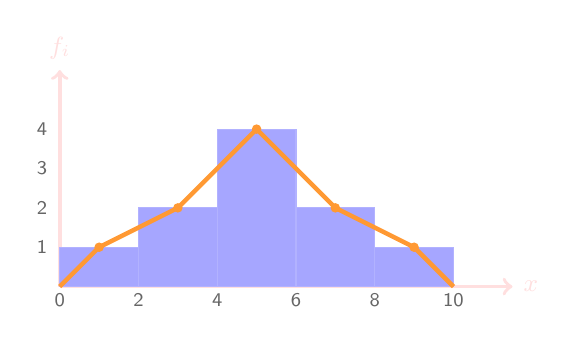
\begin{tikzpicture}[scale=0.5]
\tikzstyle{eixo}=[pink!50!white, line width=1.3pt]
\draw[eixo, ->] (0,0) -- (11.5,0) node[right, font=\small] {$x$};
\draw[eixo, ->] (0,0) -- (0,5.5)  node[above, font=\small] {$f_i$};

% barras (largura 2, alturas 1, 2, 4, 2, 1)
\fill[blue!50!white!70!white] (0,0) rectangle (2,1);
\fill[blue!50!white!70!white] (2,0) rectangle (4,2);
\fill[blue!50!white!70!white] (4,0) rectangle (6,4);
\fill[blue!50!white!70!white] (6,0) rectangle (8,2);
\fill[blue!50!white!70!white] (8,0) rectangle (10,1);
\draw[blue!30!white] (0,0) rectangle (2,1);
\draw[blue!30!white] (2,0) rectangle (4,2);
\draw[blue!30!white] (4,0) rectangle (6,4);
\draw[blue!30!white] (6,0) rectangle (8,2);
\draw[blue!30!white] (8,0) rectangle (10,1);

% polígono de frequências
\draw[orange!80!white, line width=1.6pt]
    (0,0) -- (1,1) -- (3,2) -- (5,4) -- (7,2) -- (9,1) -- (10,0);
\foreach \x/\y in {1/1, 3/2, 5/4, 7/2, 9/1}
  \filldraw[orange!80!white] (\x,\y) circle (3pt);

% eixo x — classes
\foreach \x/\l in {0/0, 2/2, 4/4, 6/6, 8/8, 10/10}
  \node[font=\scriptsize, black!60!white] at (\x,-0.35) {\l};

% eixo y — frequências
\foreach \y in {1,2,3,4}
  \node[font=\scriptsize, black!60!white] at (-0.45,\y) {\y};
\end{tikzpicture}
\end{center}

\TM{Boxplot (diagrama de caixa):}

Resume em 5 valores: mínimo, $Q_1$, mediana ($Q_2$), $Q_3$ e máximo. A caixa vai de
$Q_1$ a $Q_3$; a linha interna é a mediana; os bigodes vão ao mínimo e ao máximo.

\TM{Exemplo — dados 2, 4, 5, 6, 7, 8, 9 ($n = 7$):}

$Q_2 = 6$ (pos.\ 4) \quad $Q_1 = 4$ \quad $Q_3 = 8$

Mín = 2 \; $Q_1$ = 4 \; $Q_2$ = 6 \; $Q_3$ = 8 \; Máx = 9

$IQR = Q_3 - Q_1 = 4$

\fcolorbox{laranja}{white}{\parbox{0.85\linewidth}{
\small\textbf{Outliers:} valores fora de $[Q_1 - 1{,}5\cdot IQR,\; Q_3 + 1{,}5\cdot IQR]$
são considerados outliers e aparecem como pontos isolados no boxplot.
}}

\end{multicols}

\lfoot{\scriptsize © Copyright, Pratique Já}
\cfoot{\large \textcolor{bluebell}{pratiqueja.com}}
\end{document}
